\documentclass{article}
\newtheorem{thm}{Theorem}
\setlength{\oddsidemargin}{0.25in}
\setlength{\textwidth}{6in}
\setlength{\topmargin}{-0.25in}
\setlength{\headheight}{0.3in}
\setlength{\headsep}{0.2in}
\setlength{\textheight}{9in}
\setlength{\footskip}{0.1in}
\usepackage{multirow}
\usepackage{float}
\usepackage{fullpage}
\usepackage{graphicx}
\usepackage{amsthm}
\usepackage{amssymb}
\usepackage{url}
\usepackage{amsfonts}
\usepackage{algpseudocode}
\usepackage{mathtools}
\newcommand{\quotes}[1]{``#1''}

\usepackage{hyperref}
\hypersetup{
    colorlinks=true,
    linkcolor=blue,
    filecolor=magenta,      
    urlcolor=blue,
}

\begin{document}\title{Homework 2\\ Applied Machine Learning \\ Fall 2017\\ CSCI-P 556/INFO-I 526}         % Enter your title between curly braces
  \author{ Shradha Baranwal \\ sbaranwa@iu.edu}       % Enter your name between curly braces       % Enter your name between curly braces
\date{\today}          % Enter your date or \today between curly braces
\maketitle
\makeatother     % `@' is restored as a "non-letter" character
\pagestyle{plain}


 %%%%%%%%%%%%%%%%%%%%%%%%%%%%%%%%%%%%%%%%%%%%%%%%%%%%%

%     PROBLEM 1

 %%%%%%%%%%%%%%%%%%%%%%%%%%%%%%%%%%%%%%%%%%%%%%%%%%%%%
 
 
\section*{Problem 1 [20 points]} 

\begin{enumerate}
  \item[a)] Complete linkage hierarchical clustering\\  
  Dissimilarity Matrix :
  \[
  M=
  \left[ {\begin{array}{cccc}
    & 0.3 & 0.4 & 0.7\\
   0.3 &  & 0.5 & 0.8\\
   0.4 & 0.5 &  & 0.45\\
   0.7 & 0.8 & 0.45 & \\
  \end{array} } \right]
\]

Dissimilarity after first fusion : 
 \[
  M=
  \left[ {\begin{array}{ccc}
    & 0.5 & 0.8 \\
   0.5 &  & 0.45 \\
   0.8 & 0.45 &  \\   
  \end{array} } \right]
\]

Dissimilarity after second fusion :
  \[
  M=
  \left[ {\begin{array}{cc}
    & 0.8  \\
   0.8 &   \\  
  \end{array} } \right]
\]
    \begin{figure}[H]
    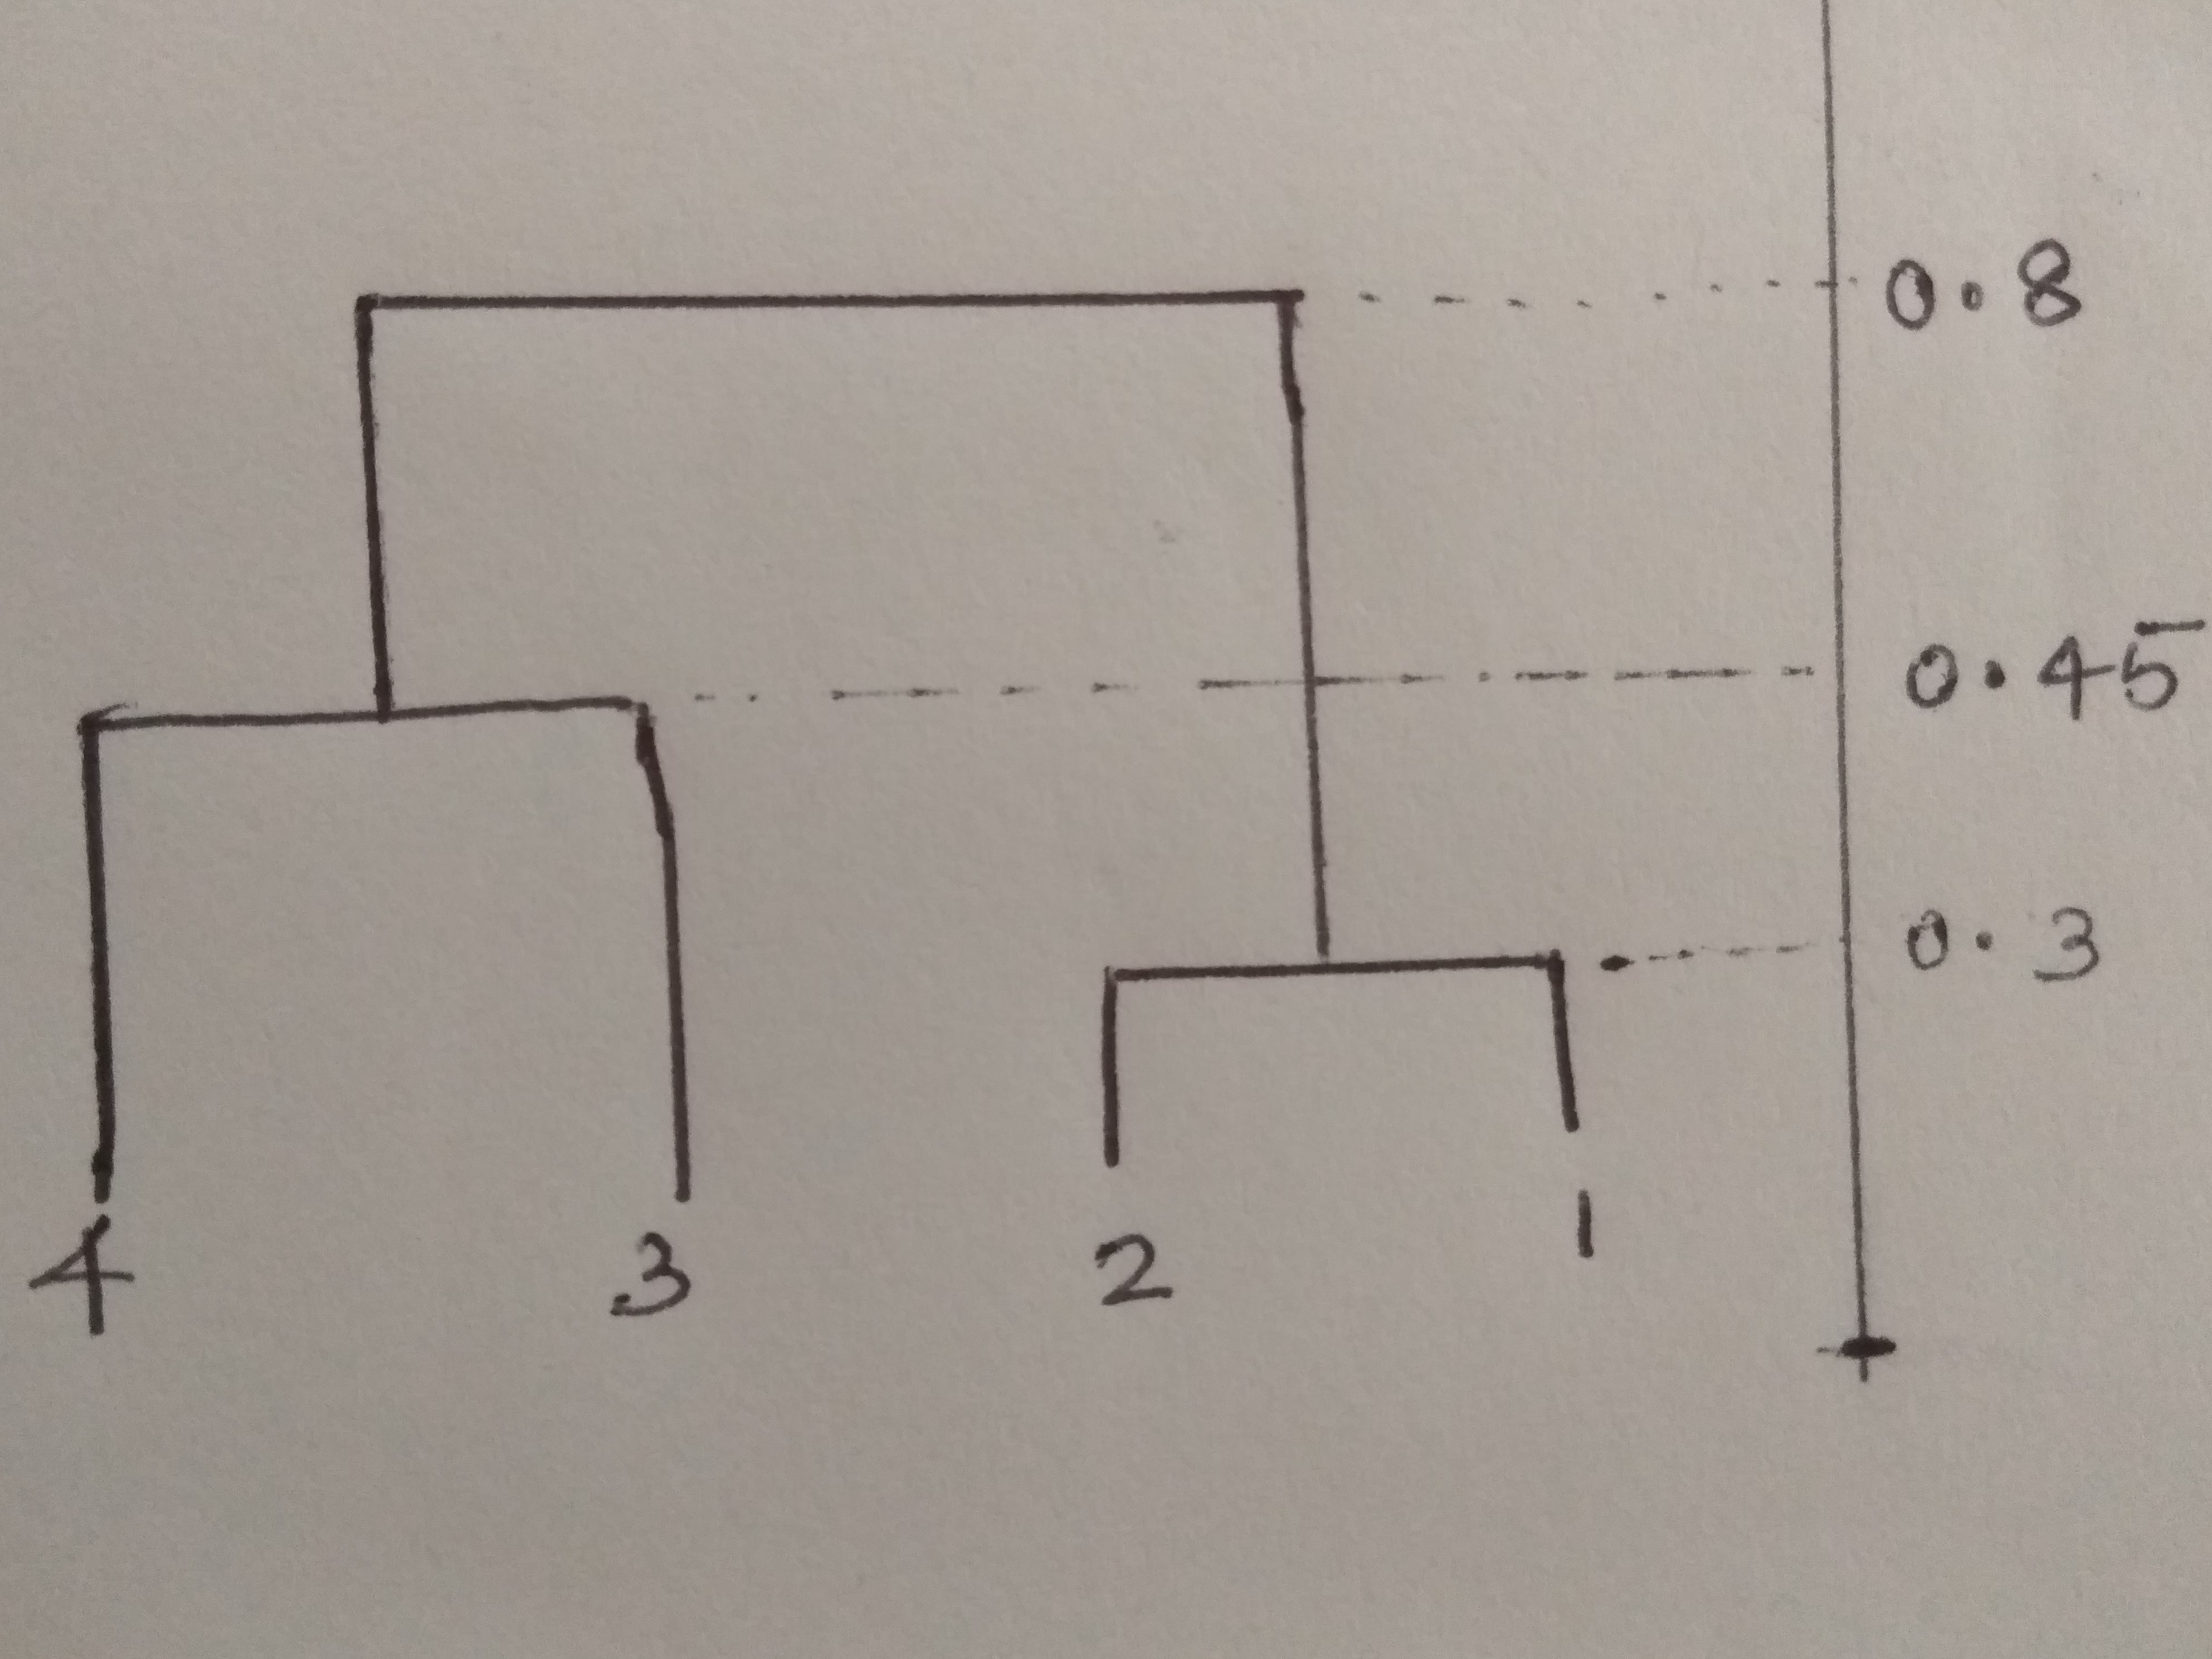
\includegraphics[width=\linewidth]{Complete_linkage.jpg}
      \caption{Complete Linkage}
  	\end{figure}    
  \item[b)] Single linkage hierarchical clustering\\
  Dissimilarity Matrix :
  \[
  M=
  \left[ {\begin{array}{cccc}
    & 0.3 & 0.4 & 0.7\\
   0.3 &  & 0.5 & 0.8\\
   0.4 & 0.5 &  & 0.45\\
   0.7 & 0.8 & 0.45 & \\
  \end{array} } \right]
\]

Dissimilarity after first fusion : 
 \[
  M=
  \left[ {\begin{array}{ccc}
    & 0.4 & 0.7 \\
   0.4 &  & 0.45 \\
   0.7 & 0.45 &  \\   
  \end{array} } \right]
\]

Dissimilarity after second fusion :
  \[
  M=
  \left[ {\begin{array}{cc}
    & 0.45  \\
   0.45 &   \\  
  \end{array} } \right]
\]
    \begin{figure}[H]
      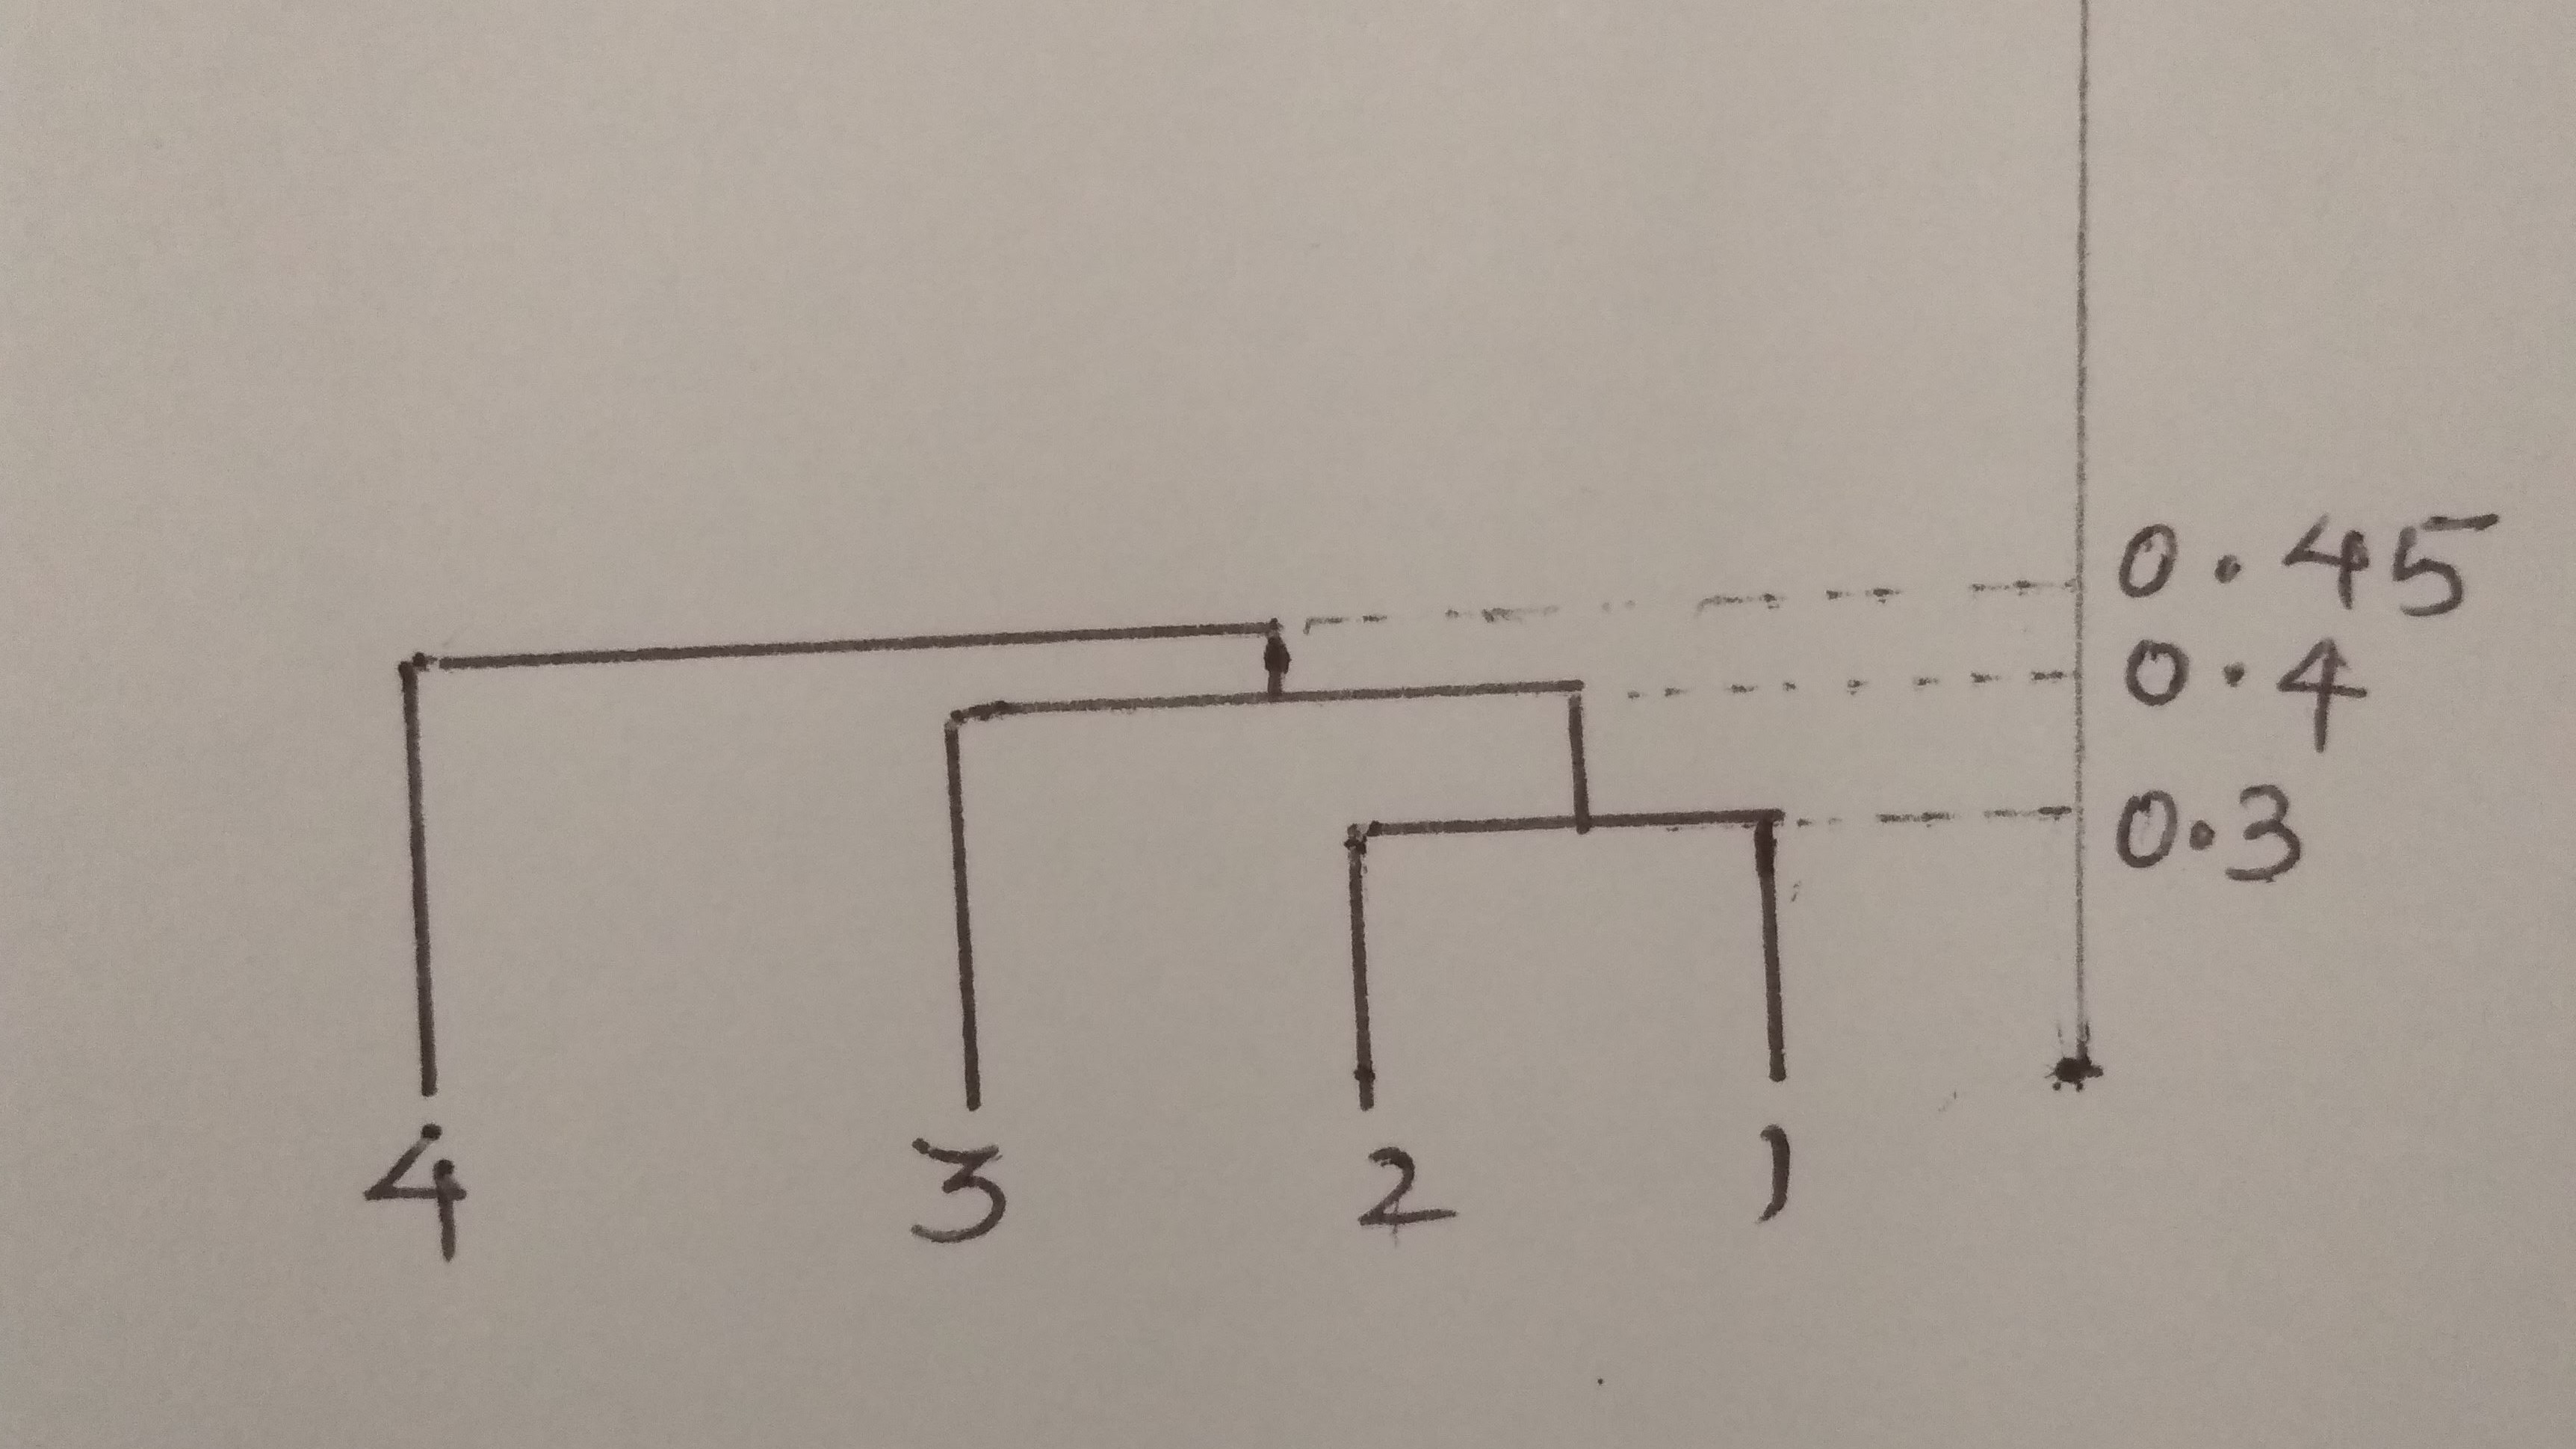
\includegraphics[width=\linewidth, scale = 0.5]
      {Single_linkage.jpg}
      \caption{Single Linkage}
  	\end{figure} 
  \item[c)]  Cutting the dendogram(a) to form two clusters\\
  In the above answer (a), on cutting the dendogram to form two clusters,
  the observations in each cluster are : (4,3), (1,2)
  
  \begin{figure}[H]
      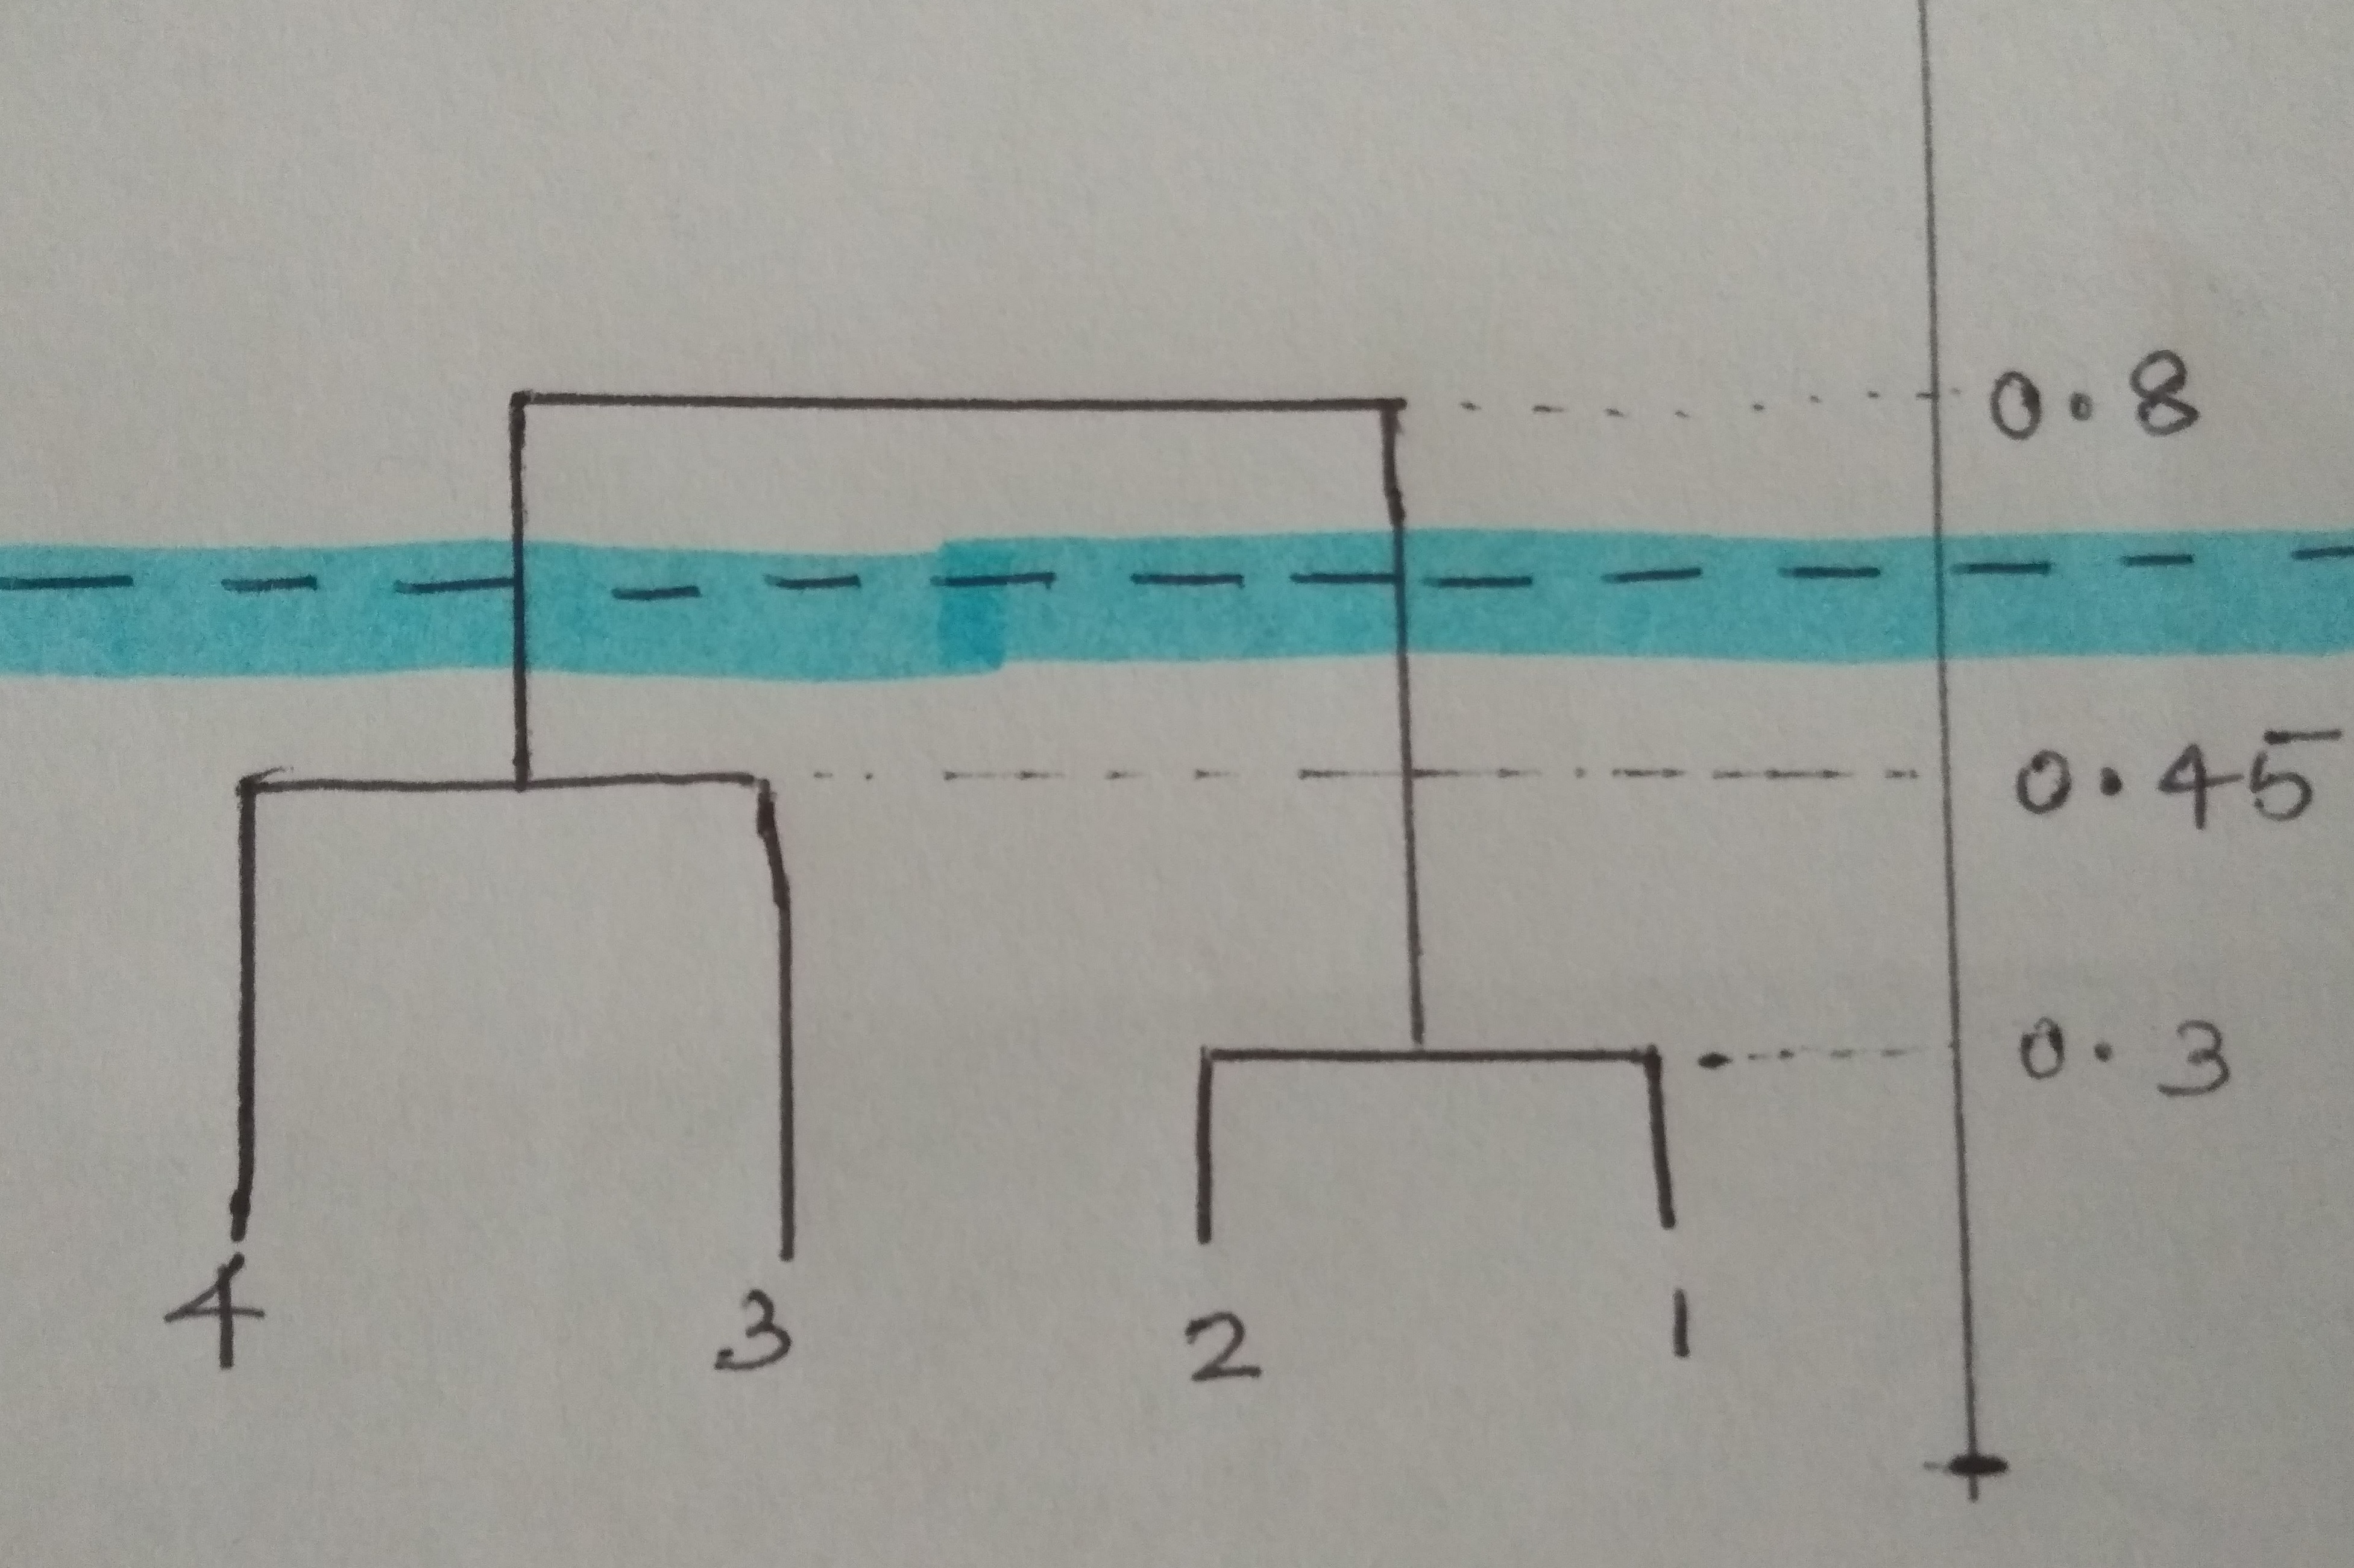
\includegraphics[width=\linewidth,scale=0.5]{2clust_comp_linkage.jpg}
      \caption{Cluster Complete Linkage}
  	\end{figure}
  
  \item[d)] Cutting the dendogram(b) to form two clusters\\
  In the above answer (b), on cutting the dendogram to form two clusters,
  the observations in each cluster are : (4), (1,2,3)
  
  \begin{figure}[H]
      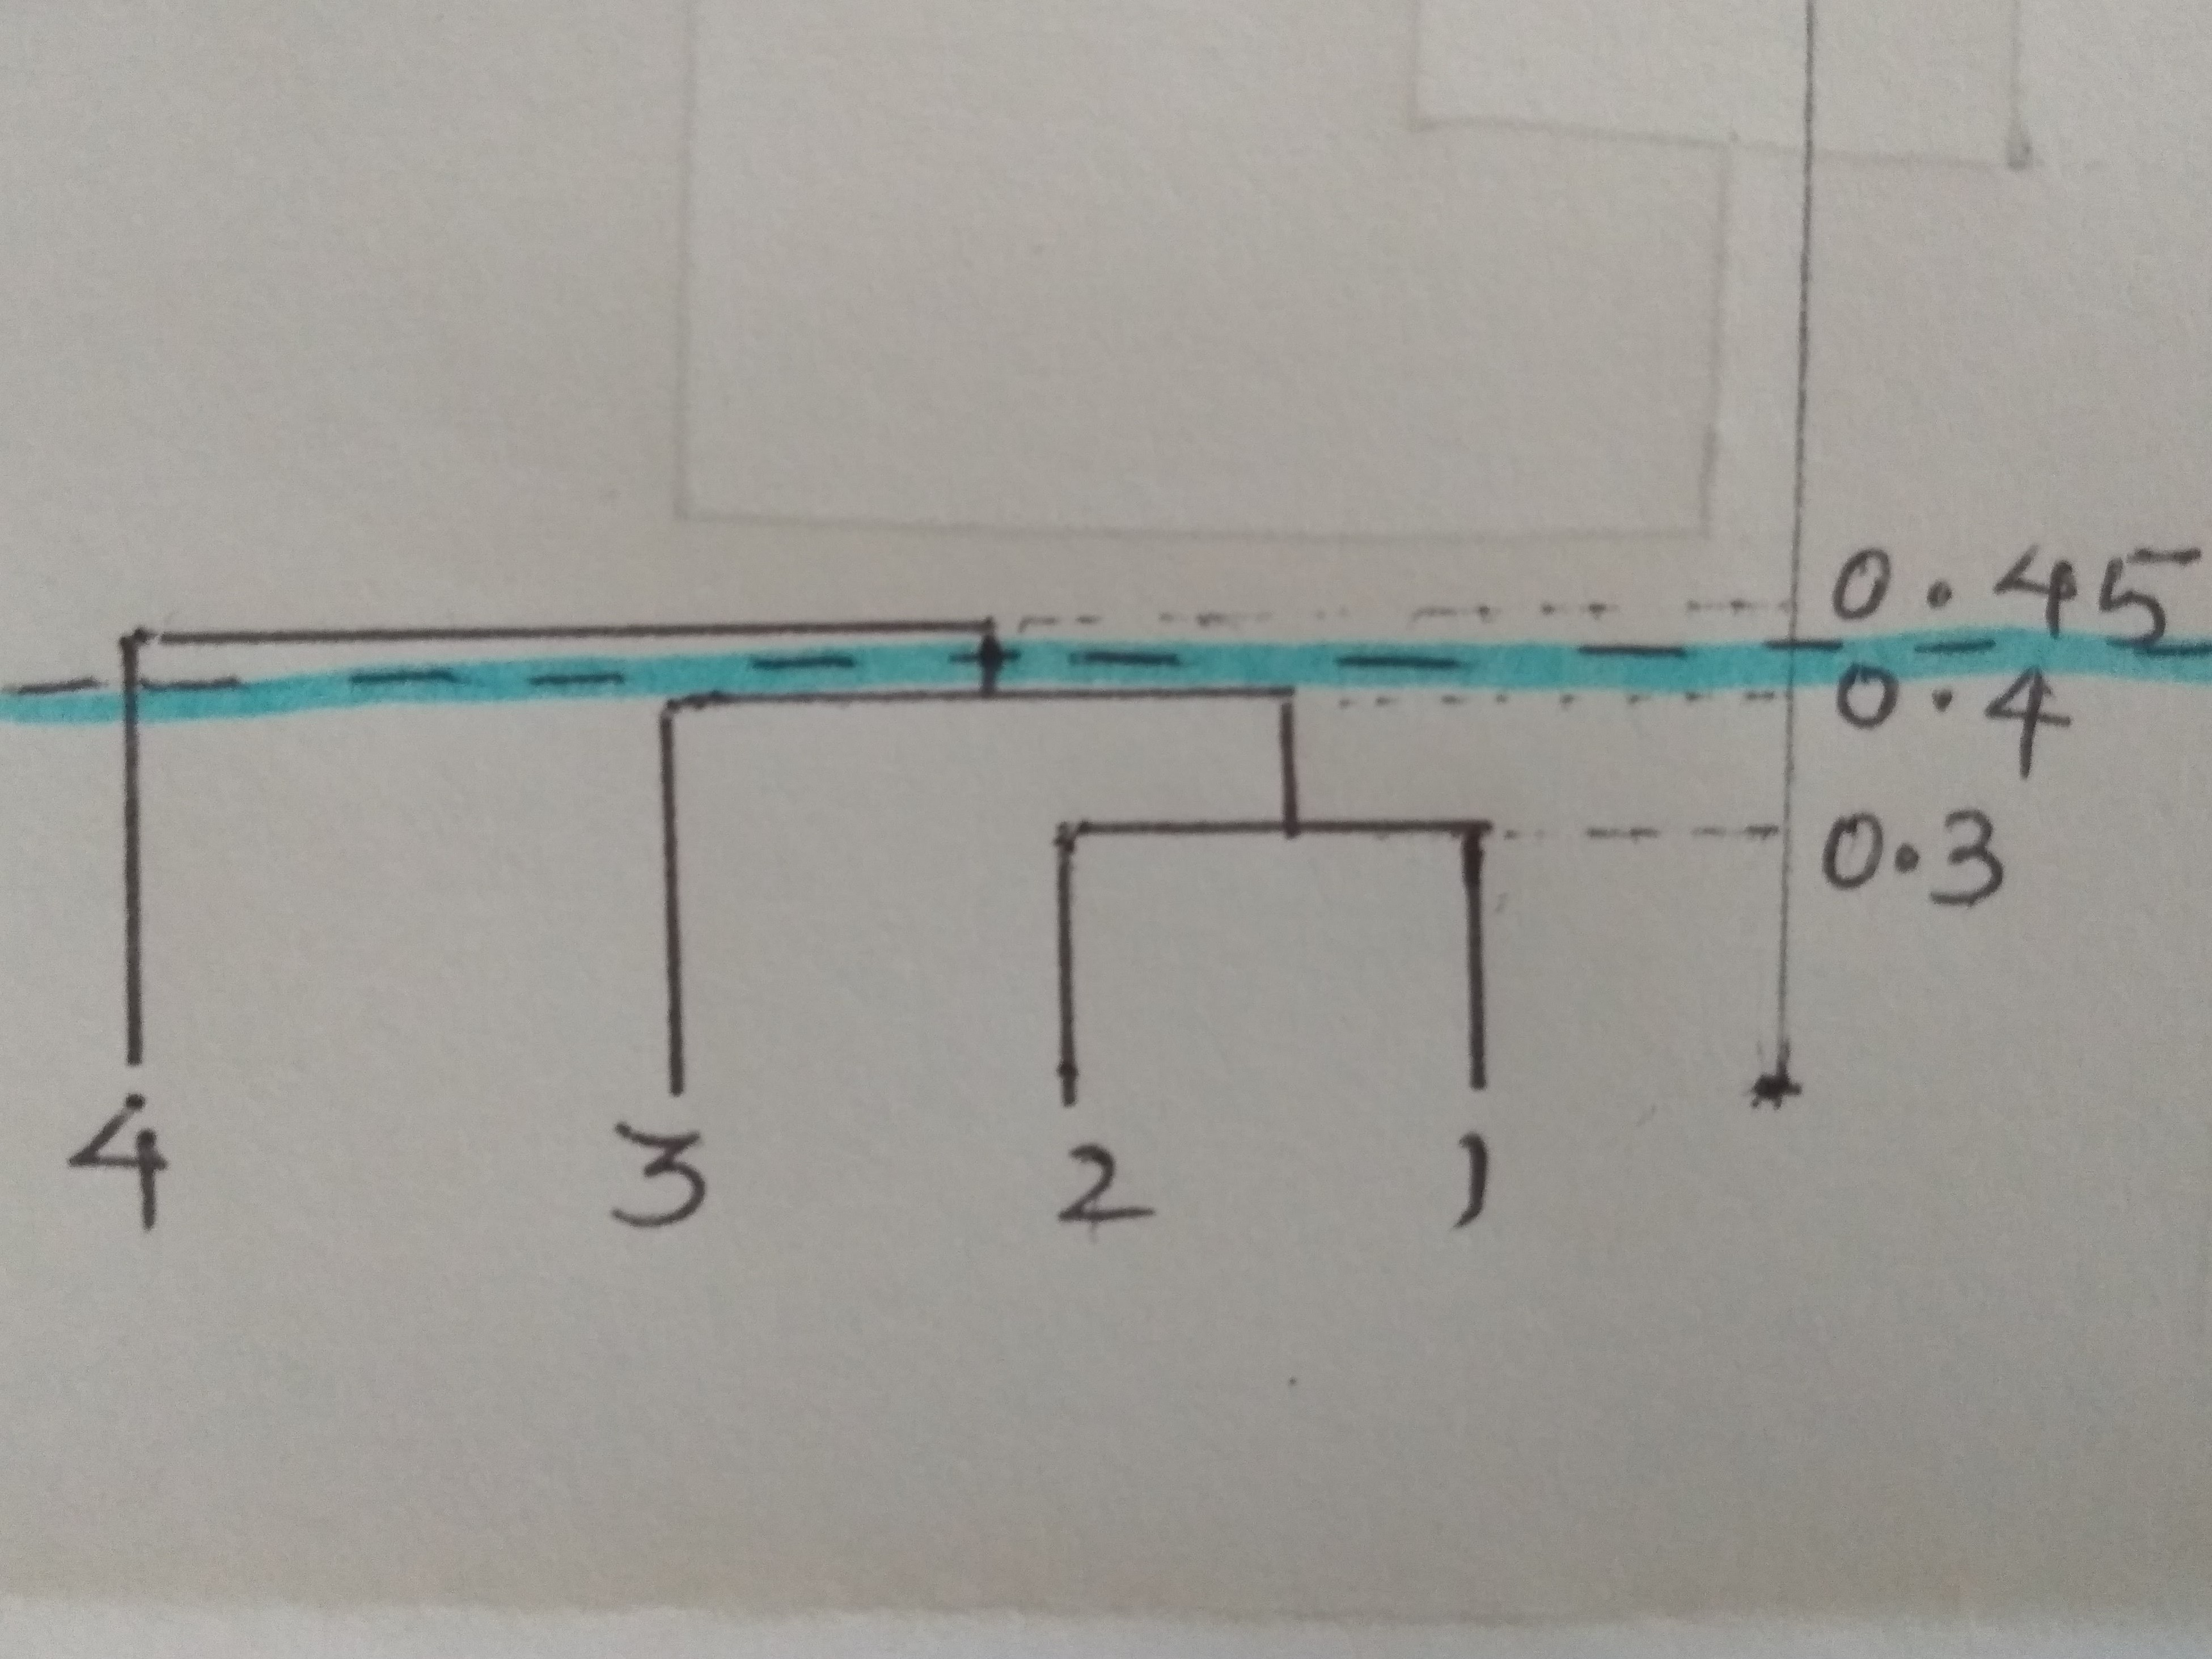
\includegraphics[width=\linewidth]{2clust_sin_linkage.jpg}
      \caption{Cluster single Linkage}
  	\end{figure}
  \item[e)] Reposition of leaves\\
  \begin{figure}[H]
     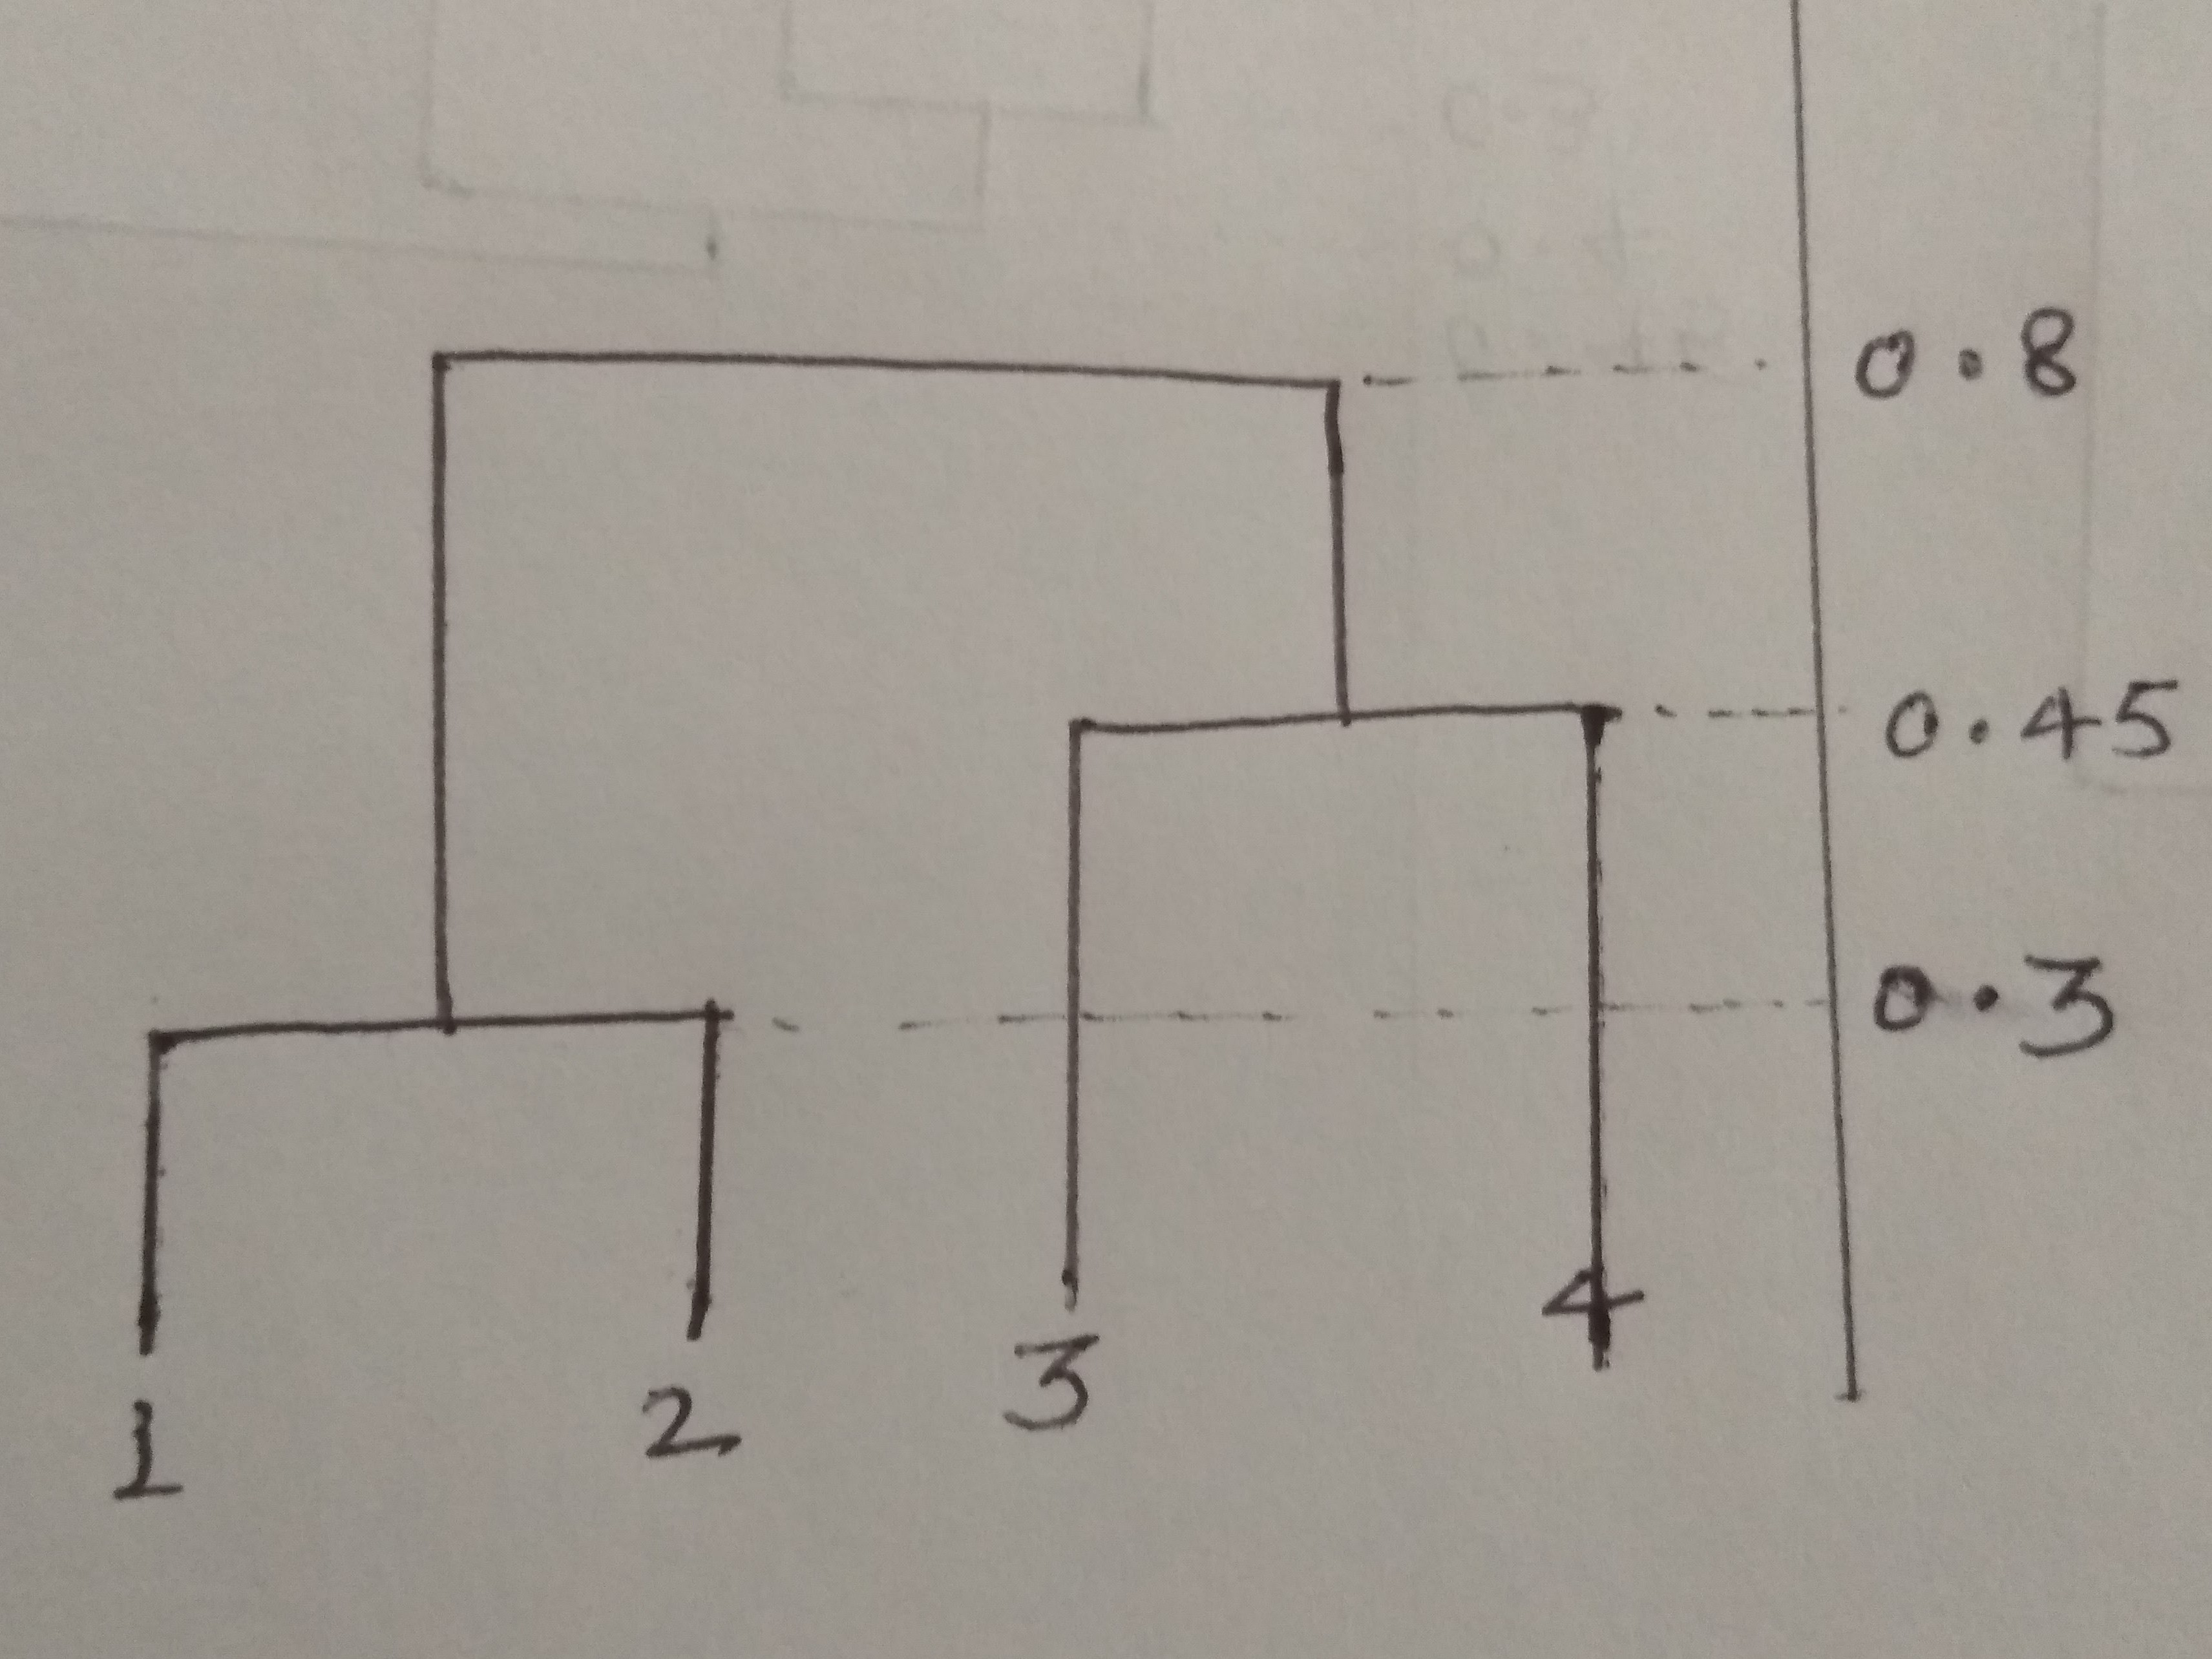
\includegraphics[width=\linewidth]
     {Reposition_leaves.jpg}
      \caption{Reposition of leaves}
  	\end{figure}
    
    Since the information of cluster dissimilarity lies on the vertical axis, repositioning of leaves in fusion doesn't change the meaning of the dendogram.
    
\end{enumerate}


 %%%%%%%%%%%%%%%%%%%%%%%%%%%%%%%%%%%%%%%%%%%%%%%%%%%%%

%     PROBLEM 2

 %%%%%%%%%%%%%%%%%%%%%%%%%%%%%%%%%%%%%%%%%%%%%%%%%%%%%


\section*{Problem 2 [50 points]} 

 Implement expectation-maximization algorithm for Gaussian mixture models (see the EM algorithm below) in \textit{R}  and call this program $G_k$. As you present your code explain your protocol for


\begin{enumerate}
  \item[2.1] Initializing each Gaussian \\
  			The three variables of a probability distribution are mean, covariance matrix and priors.\\
            Mean is initialized to random points from data set.\\
            Covariance matrix is initialized to identity matrix which is independent variables.
            Priors are initialized to uniform which is 1/k.
            
  \item[2.2] maintaining $k$ Gaussian\\
  The gaussians are updated by calculating the probabilities of each data point on each gaussian distribution. \\
  Using the normalized probabilities as weights, the mean, covariances and priors are recalculated and the cycle continues. \\
  The final gaussian distribution is decided when the sum of squared distances between means is lesser than a threshold value. 
  \item[2.3]  deciding ties\\
  In the EM implementation, I have used which.max() function to find the gaussian distribution in which the probability of a particular data point is maximum. This function returns the first index which contains the maximum value. This is basically selecting a cluster at random as the order of index for each cluster is random.
  \item[2.4] stopping criteria\\
  The threshold value for the sum of squared differences of the mean is passed as an argument to the function which is used as stopping criteria.
  In case of singular covariance matrix for jth cluster during the convergence, the  mean for jth cluster is randomly selected and covariance is set back to identity matrix. 
\end{enumerate}



 %%%%%%%%%%%%%%%%%%%%%%%%%%%%%%%%%%%%%%%%%%%%%%%%%%%%%
%PROBLEM 3

 %%%%%%%%%%%%%%%%%%%%%%%%%%%%%%%%%%%%%%%%%%%%%%%%%%%%%

\section*{Problem 3 [70 points]}

In this questions, you are asked to run your program, $G_k$, against the Ringnorm and Ionosphere data sets and compare $G_k$  with  $C_k$ ($k$-means algorithm from previous homework).  
Answer the following questions:

\begin{enumerate}
  \item[\textbf{3.1}]  Comparison between $G_k$  with  $C_k$ for ionosphere and ringnorm data sets. \\
    \begin{figure}[H]
       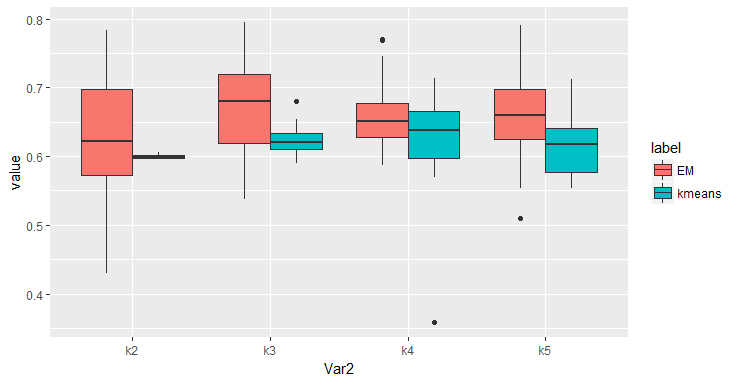
\includegraphics[width=\linewidth]{Ionosphere_3_1_error.png}
       \caption{Error comparison between EM and K means algorithm for Ionosphere dataset}
      \end{figure}

      \begin{figure}[H]
        \includegraphics[width=\linewidth]{Ionosphere_3_1_iteration.png}
        \caption{Comparison of number of iterations for K means and EM algorithms Ionosphere dataset}
      \end{figure}
      
      Looking at the error comparison graph between $G_k$  with  $C_k$ for Ionosphere dataset, the mean of the error calculated is more for EM algorithm as compared to k means algorithm. \\
      The number of iterations, however, is lesser for $G_k$ as compared to $C_k$ for the same threshold as well as same set of initial centroids.
      
    
    \begin{figure}[H]
      \includegraphics[width=\linewidth]{Ringnorm_3_1_error.png}
      \caption{Error comparison between EM and K means algorithm for Ringnorm dataset}
  	\end{figure}
    
    \begin{figure}[H]
      \includegraphics[width=\linewidth]{Ringnorm_3_1_iteration.png}
      \caption{Comparison of number of iterations for K means and EM algorithms Ringnorm dataset}
  	\end{figure}
    
    The graphs for ringnorm dataset comparing both the algorithms is similiar to the graphs generated for ionosphere data with error rate averaging higher as compared to kmeans average error. \\
    The number of iterations for EM in case of ringnorm data is lower as compared to kmeans.
  
  
  \item[\textbf{3.2}] In this question, we will run your $G_k$ with fixing the variances to ones and the priors to be uniform. Do not update the variances and priors throughout  iterations.  As explained in question 3.1,  compare  your new $G_k$  and $C_k$ using whisker plots. Discuss your results, i.e., which one performed better.
  
    \begin{figure}[H]
       \includegraphics[width=\linewidth]{Ionosphere_3_2_error.png}
       \caption{Error comparison between EM and K means algorithm for Ionosphere dataset}
      \end{figure}

      \begin{figure}[H]
        \includegraphics[width=\linewidth]{Ionosphere_3_2_iteration.png}
        \caption{Comparison of number of iterations for K means and EM algorithms}
      \end{figure}
    
    \begin{figure}[H]
      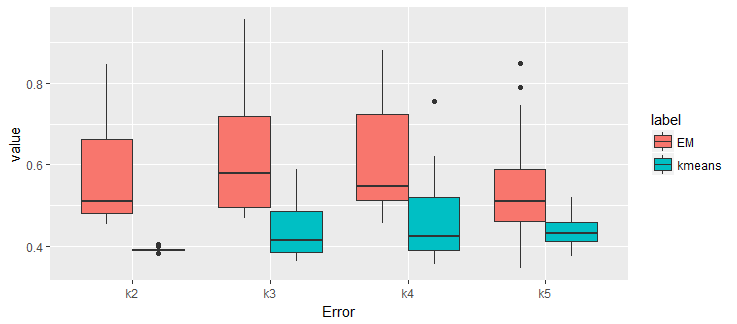
\includegraphics[width=\linewidth]{Ringnorm_3_2_error.png}
      \caption{Error comparison between EM and K means algorithm for Ringnorm dataset}
  	\end{figure}
    
    \begin{figure}[H]
      \includegraphics[width=\linewidth]{Ringnorm_3_2_iteration.png}
      \caption{Comparison of number of iterations for K means and EM algorithms}
  	\end{figure}
  
 After keeping constant the co variances and mean of gaussian distributions in EM algorithm, there was not much difference in the error and number of iterations graphs for Ionosphere dataset. 
 However, in case of ringnorm dataset, the mean error for ringnorm dataset increased for EM increased as compared to the last time. However, the number of iterations remained lower than the k means. 
  
\end{enumerate}
 
 %%%%%%%%%%%%%%%%%%%%%%%%%%%%%%%%%%%%%%%%%%%%%%%%%%%%%
 

  %%%%%%%%%%%%%%%%%%%%%%%%%%%%%%%%%%%%%%%%%%%%%%%%%%%%%
%PROBLEM 4

 %%%%%%%%%%%%%%%%%%%%%%%%%%%%%%%%%%%%%%%%%%%%%%%%%%%%%

 
  \section*{Problem 4 [50 points]}  
  
In this question, you will first perform principal component analysis (PCA) over Ionosphere and Ringnorm data sets and then cluster the  reduced data sets using $G_k$ (from question 3.1) and $C_k$. You are allowed to use R packages for PCA.
Ignore the class variables (35th and 1st variables for Ionosphere  and Ringnorm data sets, respectively) while performing PCA. Answer the questions below:
 \\
  \begin{enumerate}
  \item[\textbf{4.1}]  Make a scatter plot of PC1 and PC2  for both data sets. Discuss principal
components (The first and  second principal components). What are PC1 and PC2?
\\
\begin{figure}[H]
      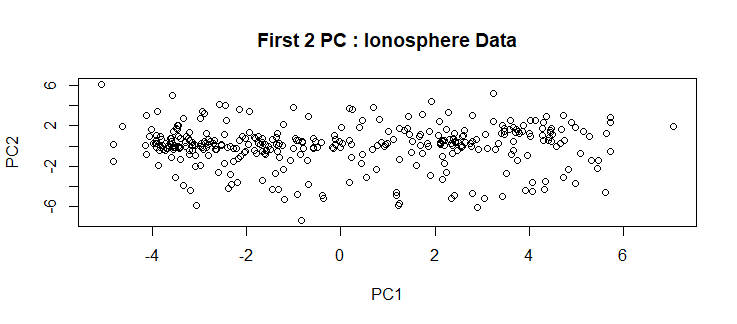
\includegraphics[width=\linewidth]{Ionosphere_PC5_scatter.png}
      \caption{Scatter plot of first 2 principal components for ionosphere data}
  	\end{figure}
    
    \begin{figure}[H]
      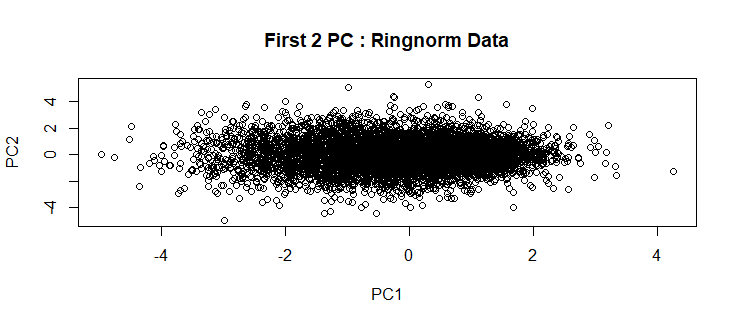
\includegraphics[width=\linewidth]{Ringnorm_PC5_scatter.png}
      \caption{Scatter plot of first 2 principal components for ringnorm data}
  	\end{figure}

The first two principal component vectors of any data set gives the plane from which the data points are the closest. Hence, the variance maintained by these 2 principal component vectors is the maximum of all the principal components.
The first two principal component score vectors are the projections of each data point on the plane principal component vectors 1 and 2.

  \item[\textbf{4.2}]  Create scree plots after PCA and explain the plots.
\\
	\begin{figure}[H]
      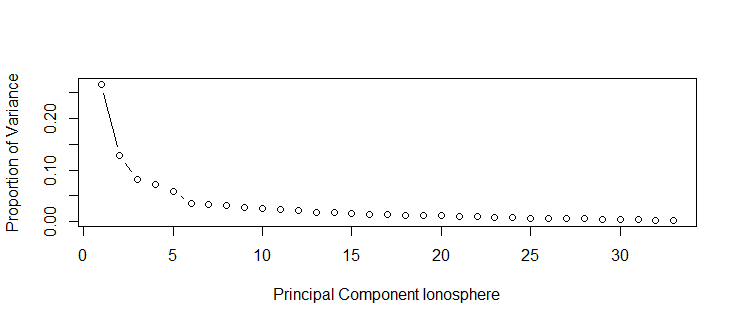
\includegraphics[width=\linewidth]{Ionosphere_pca_variance.png}
      \caption{Scree plot Ionosphere Data}
  	\end{figure}
    
    \begin{figure}[H]
      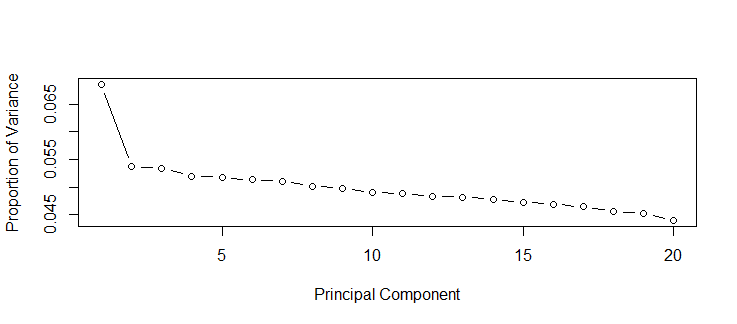
\includegraphics[width=\linewidth]{Ringnorm_pca_variance.png}
      \caption{Scree plot Ringnorm Data}
  	\end{figure}
    
The above two figures gives the percentage of variance of each pc for both ionosphere and ringnorm data set. The variances in ionosphere dataset is a monotonically decreasing graph wherein the variance help by the last few pc are tending to zero.\\
In case of ringnorm data, however, the percentage of variance is pretty small in the first pc and decreases almost linearly. 

\begin{figure}[H]
      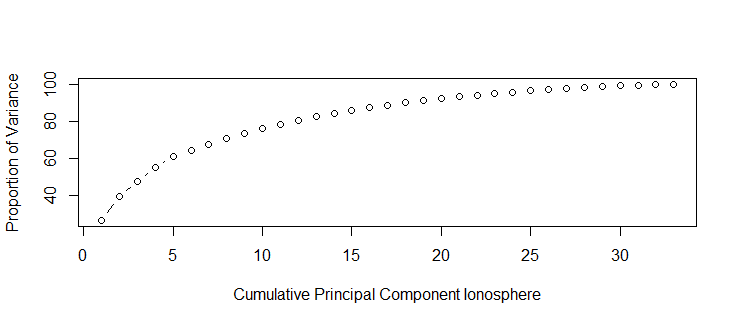
\includegraphics[width=\linewidth]{Ionosphere_pca_cumvar.png}
      \caption{Scree plot Ionosphere Data}
  	\end{figure}
    
    \begin{figure}[H]
      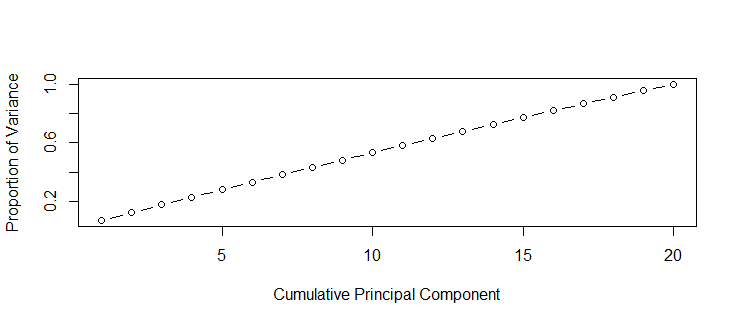
\includegraphics[width=\linewidth]{Ringnorm_pca_cumvar.png}
      \caption{Scree plot Ringnorm Data}
  	\end{figure}
The above figures show the cumulative variance of each principal component for both ionosphere and ringnorm data sets. 
The variance of each principal component in ionosphere dataset is decreasing. However, in case of ringnorm the variance of each principal component is almost same. Hence, to maintain 90\% of the variance in both the data sets, 12 PCs can be dropped reducing the number of variables to 19. However, in case of ringnorm, to maintain the same percentage of variance, only few PCs could be excluded.




  \item[\textbf{4.3}]  Observe the loadings using prcomp() or princomp() functions in R and  discuss loadings in PCA?i.e., how are principal components and original variables related?\\
\\
The principal loadings vectors are the directions in the feature space with the maximum variance of data. There can be a maximum of d (number of dimensions and $d < n$) principal components. They are the planes which are closest to the data using Euclidean distance metric.\\
The loadings are vectors which are used to calculate the projections of data in a that direction. The projections are the principal component score vectors. Each principal component gives the variance of the data maintained in that component in the decreasing order.\\
Thus, you can say that the principal components score vectors are the projections of original variables in the direction of principal components vectors.


  \item[\textbf{4.4}]  Keep $90\%$ of variance  after PCA and reduce Ionosphere and Ringnorm data sets.  Run $C_k$ and $G_k$ with the reduced data sets and compare them using whisker plots as shown in question 3.1\\
 \\
 Below are the comparison graphs of error and iteration for ringnorm and ionosphere datasets after reducing the variables by keeping 90\% variance of data :
  
 \begin{figure}[H]
       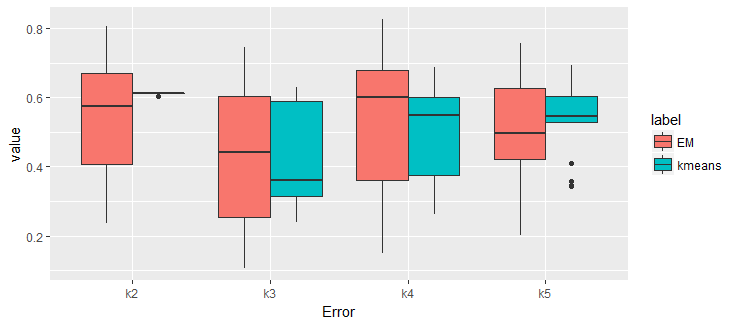
\includegraphics[width=\linewidth]{Ionosphere_pca4_error.png}
       \caption{Error comparison between EM and K means algorithm for Ionosphere dataset}
      \end{figure}

      \begin{figure}[H]
        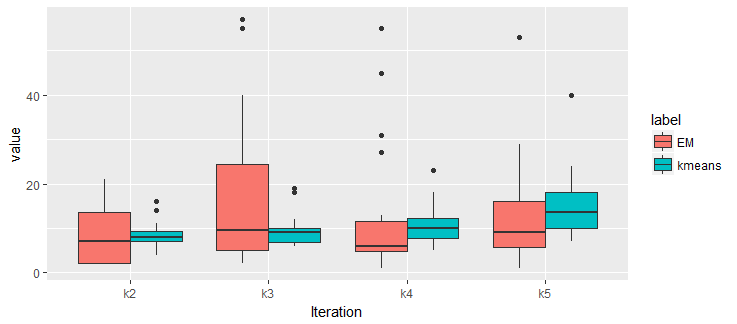
\includegraphics[width=\linewidth]{Ionosphere_pca4_iteration.png}
        \caption{Comparison of number of iterations for K means and EM algorithms}
      \end{figure}
    
    \begin{figure}[H]
      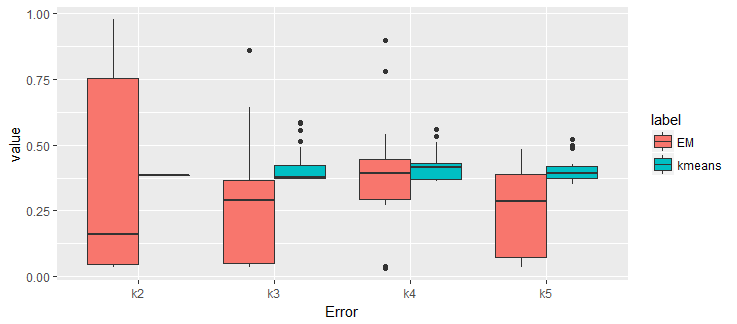
\includegraphics[width=\linewidth]{Ringnorm_pca4_error.png}
      \caption{Error comparison between EM and K means algorithm for Ringnorm dataset}
  	\end{figure}
    
    \begin{figure}[H]
      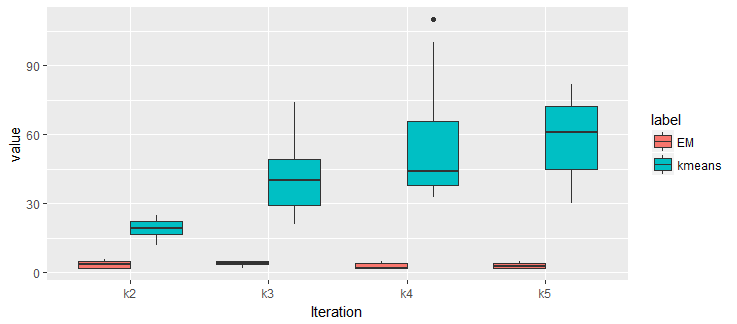
\includegraphics[width=\linewidth]{Ringnorm_pca4_iteration.png}
      \caption{Comparison of number of iterations for K means and EM algorithms}
  	\end{figure}
    
In case of ionosphere, the number of iterations has reduced significantly. This might be due to the reduction of number of variables significantly. However, the graph for number of iterations for ringnorm has remained the same as without pca. This is because the number of variables has not reduced much in case of ringnorm data.

 
  \item[\textbf{4.5}] Discuss that how PCA affects the performance of $C_k$ and $G_k$.  
\end{enumerate}

  %%%%%%%%%%%%%%%%%%%%%%%%%%%%%%%%%%%%%%%%%%%%%%%%%%%%%
%                      PROBLEM 5

 %%%%%%%%%%%%%%%%%%%%%%%%%%%%%%%%%%%%%%%%%%%%%%%%%%%%%

 
 \section*{Problem 5 [50 points]}  Randomly choose 50 points from Ionosphere data set (call this data set $\text{I}_{50}$) and perform hierarchical clustering. You are allowed to use R packages for this question. (Ignore the class variable while performing hierarchical clustering.)
 \\ 
 
 \begin{enumerate}
  \item[\textbf{5.1}]  Using hierarchical clustering with complete linkage and Euclidean distance cluster $\text{I}_{50}$. Plot the dendrogram.
\\ 

\begin{figure}[H]
      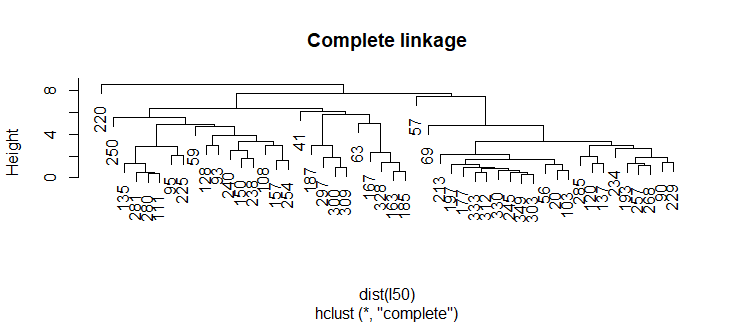
\includegraphics[width=\linewidth]{Complete_linkage_hc5.png}
      \caption{Complete linkage for $\text{I}_{50}$}
  	\end{figure}
    
     
\item[\textbf{5.2}] Cut the dendrogram at a height that results in two distinct  clusters. Calculate an error rate.
\\  Cutting the dendogram for 2 clusters, resulted in a cluster with one element and another cluster with 49 elements.
The error rate for these cluster is : 0.3061224


  \item[\textbf{5.3}] First, perform PCA on $\text{I}_{50}$ (Keep $90\%$ of variance ). Then hierarchically cluster the reduced data using complete linkage and Euclidean distance. Plot the dendrogram.
\\  
  \begin{figure}[H]
      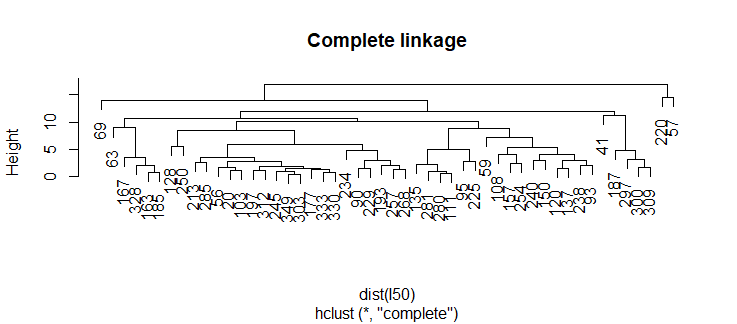
\includegraphics[width=\linewidth]{hc_pca5_3.png}
      \caption{Complete linkage 90\% variance of $\text{I}_{50}$}
  	\end{figure}
  
    \item[\textbf{5.4}]  Cut the dendrogram at a height that results in two distinct  clusters. Calculate an error rate. How  did PCA affect hierarchical clustering?
    Cutting the dendogram for 2 clusters, resulted in a cluster with two element and another cluster with 48 elements.
The error rate for these cluster is : 0.2916667
PCA resulted in the reduction of error rate after hierarchical clustering.
    
    
    
\end{enumerate}
 



 %%%%%%%%%%%%%%%%%%%%%%%%%%%%%%%%%%%%%%%%%%%%%%%%%%%%%

%      EXTRA CREDIT

 %%%%%%%%%%%%%%%%%%%%%%%%%%%%%%%%%%%%%%%%%%%%%%%%%%%%%

\section*{Extra credit [60 points]}

This part is optional. 

\begin{enumerate}
\item[\textbf{1}] Improve the EM algorithm  through initialization.  \href{http://ilpubs.stanford.edu:8090/778/1/2006-13.pdf}{$k$-means ++} is an extended $k$-means clustering algorithm and induces non-uniform  distributions over  the data  that serve as  the initial centroids. Read the paper and implement this idea to improve your $G_k$ program (from question 3.1). Run your new $G_k$ and old one (question 3.1) for $k= 2,\dots,5$ and compare the results using whisker plots. [30 points]
\\ 
\\
\begin{figure}[H]
       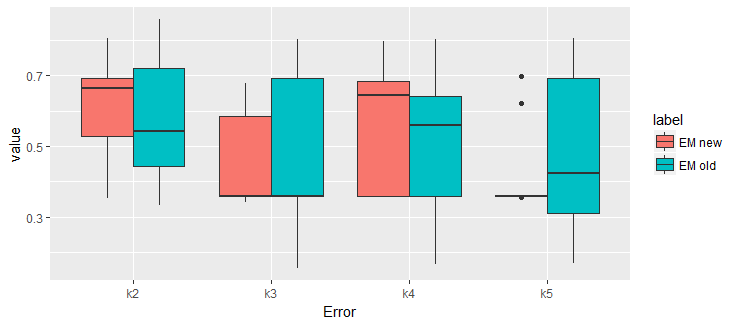
\includegraphics[width=\linewidth]{Extra_error_diff.png}
       \caption{Error comparison between EM and K means algorithm for Ionosphere dataset}
      \end{figure}

      \begin{figure}[H]
        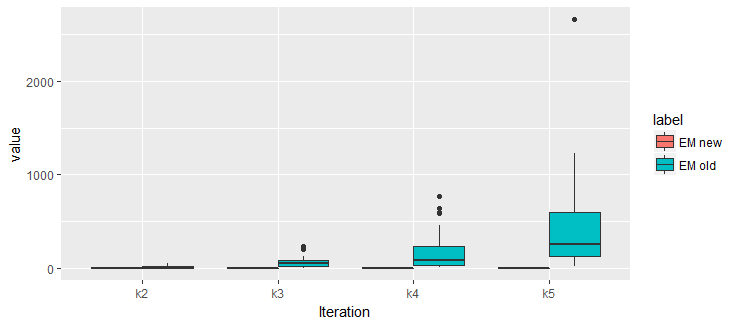
\includegraphics[width=\linewidth]{Extra_Iteration_diff.png}
        \caption{Comparison of number of iterations for K means and EM algorithms}
      \end{figure}

In the above whisker plots for error and iteration comparison between EM and EM++, the mean error difference between both the algorithms is not much. However, the number of iterations for EM++ is less. Also, the number of iterations has almost remained constant as the number of clusters increased unlike for EM in which the number of iterations increased with number of clusters.


\item[\textbf{2}]  Run the EM algorithm for different mixture models, i.e., Poisson,  and against different data sets. [30 points]
\end{enumerate}




%%%%%%%%%%%%%%%%%%%%%%%%%%%%%%%%%%%%%%%%%%%%%%%%%%%%%


%%%%%%%%%%%%%%%%%%%%%%%%%%%%%%%%%%%%%%%%%%%%%%%%%%%%%
\end{document}


